
\section{RapidWright API}
\label{sec:rapidwright_api}

\textbf{RapidWright} is an open-source Java framework from AMD/Xilinx that provides direct access to the netlist and device databases used by vendor tools. 
This framework positions itself as an additional workflow column, allowing users to intercept or replace stages of the standard design flow with custom optimization stages (see Figure~\ref{fig:vivado_dcps}).

\begin{itemize}
\item \textbf{Design Checkpoints:} 
    RapidWright leverages \texttt{.dcp} files (design checkpoints) generated at various stages of a Vivado flow. 
    By importing a checkpoint, engineers can manipulate the netlist, placement, or routing externally, then re-export a modified checkpoint for further processing in the Vivado workflow column.

\item \textbf{Key Packages:} 
    RapidWright revolves around three primary data model packages:
    \begin{enumerate}
    \item \emph{edif} -- Represents the logical netlist in an abstracted EDIF-like structure.
    \item \emph{design} -- Contains data structures for the physical implementation (Cells, Nets, Sites, BELs, etc.).
    \item \emph{device} -- Provides a database of the target FPGA architecture (e.g., Site coordinates, Tile definitions, routing resources).
    \end{enumerate}

\item \textbf{Interfacing with the Netlist and Device:} 
    An engineer can query the netlist to find specific resources (LUTs, FFs, DSPs, etc.) and then map or move them onto device sites. 
    This level of control over backend resources is necessary for research in custom placement, advanced packing techniques, or experimental routing algorithms.
\end{itemize}

{
    \centering
    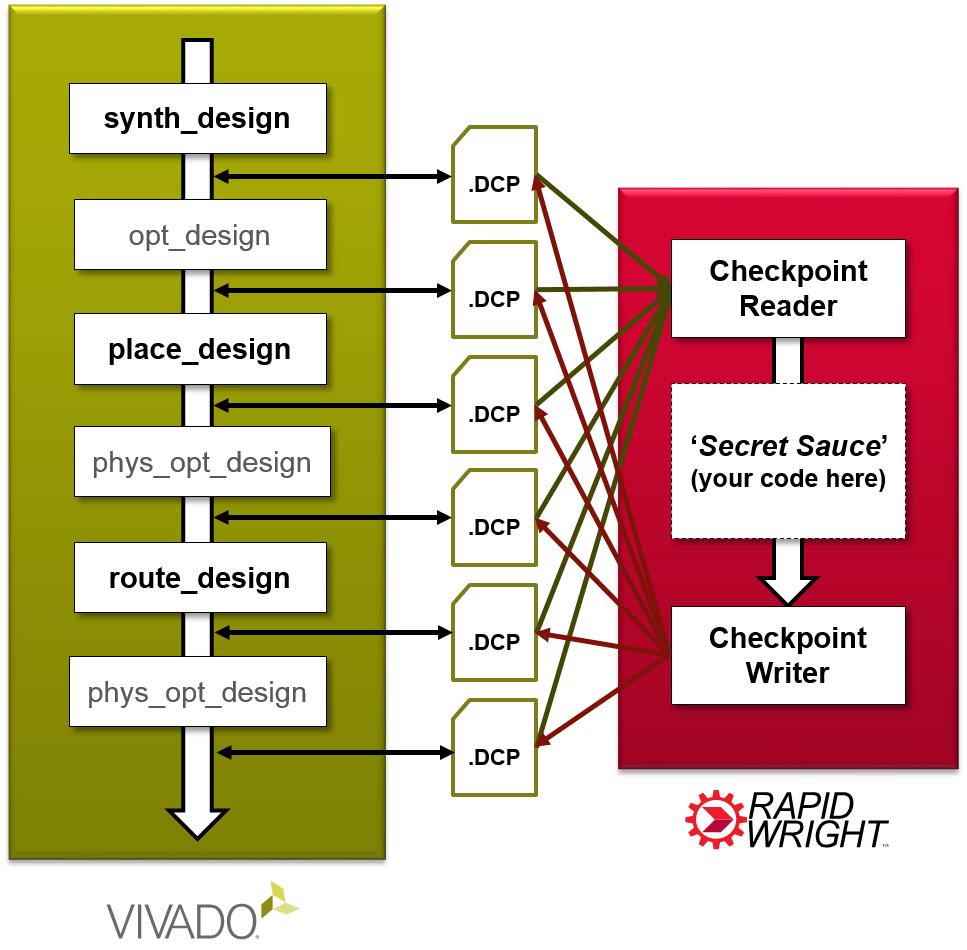
\includegraphics[width=0.8\columnwidth]{figures/vivado_dcps.png}
    \captionof{figure}{RapidWright workflow integrating into the default Vivado design flow.}
    \label{fig:vivado_dcps}
}

By exposing these low-level internals, RapidWright allows fine-grained design transformations that go beyond the standard Vivado IDE’s capabilities. 
Researchers can prototype new EDA strategies without needing to re-implement an entire FPGA backend from scratch, thus accelerating innovation in placement and routing methodologies.

